\scanpage{107}
% Archive foliation: 108.
? \uline{Proof of 1\textsuperscript{st} conj.} :

\textcircled{1} Given
\[
0\longrightarrow\Phi'\longrightarrow\Phi(G)\longrightarrow\Phi''\longrightarrow0
\]
(Galois-devissage), then can define $G'$, $G''$
so $\Phi'=\Phi(G')$, \uline{$\Phi''=\Phi(G'')$}

\deleted{$\unsure{f^j x-fy}$}
\[
\begin{array}{cccc}
f^j x=0&x=fy&x=f^2z&x=f^{n-j\unsure{-1}}t\\
&f^{j+1}y=0&y=fz&f^{n-1}t=0\\
&&f^{j+2}z=0&
\end{array}
\]
\[
\operatorname{Ker}f^j=\operatorname{Im}\qquad
\operatorname{Ker}f=\operatorname{Im}f^{n-1}
\]
\margin{$\supset$ \unsure{triv.}\quad $\subset$ hyp}
\diagram{\begin{tikzcd}
\operatorname{Ker}f^j=\operatorname{Im}f^{n-j}\arrow[d,Rightarrow,"?"]\\
\operatorname{Ker}f^{j+1}=\operatorname{Im}f^{n-j-1}
\end{tikzcd}}
\[
f^{j+1}x=0\qquad
\left\{\begin{array}{l}fx\in\operatorname{Ker}f^j\\fx=f^{n-j}y\end{array}\right.
\]
\[
\unsure{f^{-1}}(\deleted{\unsure{f}}\inserted{f^{n-j}}A)=f^{n-j-1}A
\]

\margin{
\diagram{\begin{tikzcd}
\operatorname{Ker}f^j=\operatorname{Im}f^{n-j}\arrow[d,Rightarrow]\\
\operatorname{Ker}f^{j-1}=\operatorname{Im}f^{n-j\unsure{+1}}
\end{tikzcd}}
$f^{j-1}x=0\Longrightarrow f^j x=0\qquad x=f^{n-j}y\quad\deleted{\unsure{f}}$
$f^{j-1}x=f^{n-1}y=0$
i.e. $f^j(\overbrace{f^{n-1-j}y}^{f^{n-j}z})=0$
\deleted{$\unsure{f^{n-j}y=0}$}
}

\margin{
$n=3\qquad f^3=0$
\[
\operatorname{Ker}f=\operatorname{Im}f^2
\]
$f^{j-1}x=0\qquad f^j x=0\qquad x=fy\qquad f.$
\[
A/f^2A\xrightarrow[\sim]{f}fA
\]
\[
fA/f^2A\xrightarrow{\sim}f^2A
\]
\deleted{$\unsure{A/fA}$}
\[
(f^j)^{-1}(f^{n-1}(A))=fA
\]
$\operatorname{Ker}f^j$
}

\figure{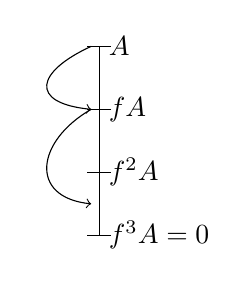
\begin{tikzpicture}[x=1cm,y=.8cm]
\draw(0,0)--(0,3);\foreach \y in {0,1,2,3}{\draw(-.15,\y)--(.15,\y);}
\node[right]at(0,3){$A$};\node[right]at(0,2){$fA$};\node[right]at(0,1){$f^2A$};\node[right]at(0,0){$f^3A=0$};
\draw[->](-.1,3)..controls(-.8,2.6)and(-.9,2.1)..(-.1,2);
\draw[->](-.1,2)..controls(-.8,1.5)and(-.9,.6)..(-.1,.5);
\end{tikzpicture}}

\figure{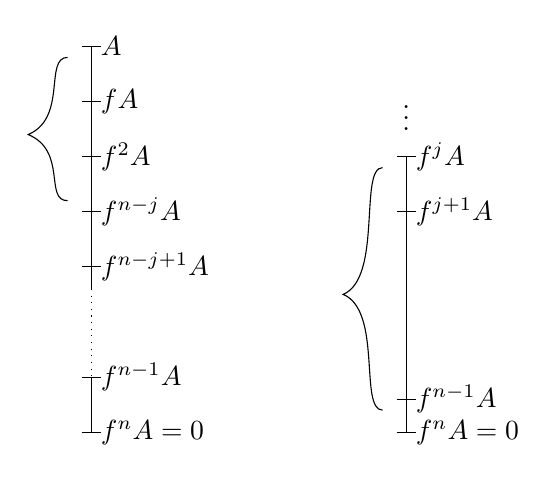
\begin{tikzpicture}[x=1cm,y=.7cm]
\draw(0,7)--(0,3);\draw(0,3)--(0,2.6);\draw[dotted](0,2.6)--(0,1);\draw(0,1)--(0,0);
\foreach \y in {0,1,3,4,5,6,7}{\draw(-.12,\y)--(.12,\y);}
\node[right]at(0,7){$A$};\node[right]at(0,6){$fA$};\node[right]at(0,5){$f^2A$};\node[right]at(0,4){$f^{n-j}A$};\node[right]at(0,3){$f^{n-j+1}A$};\node[right]at(0,1){$f^{n-1}A$};\node[right]at(0,0){$f^nA=0$};
\draw(-.3,6.8)..controls(-.6,6.8)and(-.3,5.7)..(-.8,5.4)..controls(-.3,5.1)and(-.6,4.2)..(-.3,4.2);
\draw(4,0)--(4,5);\foreach \y in {0,.6,4,5}{\draw(3.88,\y)--(4.12,\y);}
\node[above]at(4,5.3){$\vdots$};\node[right]at(4,5){$f^jA$};\node[right]at(4,4){$f^{j+1}A$};\node[right]at(4,.6){$f^{n-1}A$};\node[right]at(4,0){$\unsure{f^nA=0}$};
\draw(3.7,4.8)..controls(3.4,4.8)and(3.7,2.8)..(3.2,2.5)..controls(3.7,2.2)and(3.4,.4)..(3.7,.4);
\end{tikzpicture}}
